\chapter{Introduction}
This thesis has the goal to implement an advanced and refined version of the predecessor implementation (see \cite{korniowski}) for a fail-safe mesh network prototype using embedded technologies. This goal can be split in the following aspects:
\begin{itemize}
\item \textbf{Hardware: } The goal is to explore alternative, enhanced and reusable hardware solutions for an embedded implementation.
\item \textbf{Algorithms :} The goal is to explore and elaborate on enhanced algorithms and data structures.
\item \textbf{Simulation :} The goal is to provide the basis for a simulation environment for the provided algorithms that can execute on regular PCs.
\end{itemize}

The author wants to prove that an implementation of a robust and scalable mesh network using embedded devices despite its hardware constraints is quite possible. He wants to explore algorithms and software architectures usually hidden behind the curtain of operating systems.
The desired end result is not only to have a working mesh network prototype but also an algorithmic framework for further development. Therefore the author also wanted to provide a framework which allows to try and research future algorithms on a regular PC.
Finally the author wanted to provide a reproducible hardware design in order to able to equip a complete laboratory of mesh nodes for further research and investigation.

\section{Thesis overview}
The thesis is structured in the same order as the above mentioned goals. The first part analyzes the existing prototype hardware. An enhanced version is proposed by providing an alternative CPU and the connection of external RAM. Level shifters are introduced for the connection of the RFM12B radio module and the existing UART connection is being enhanced by an USB interface. Finally connectors for an external keyboard and an external LCD module are introduced.

The second part elaborates on the envisioned software architecture. It identifies the necessary software modules which have to be implemented in order to provide a robust design. It defines modules for the human interaction and for the internal state control. The network stack module and the RFM12B driver module are identified for the mesh network access.

The third part explores the algorithmic foundations and data structures which are being used for the implementation. Different concurrency models are being analyzed and a threading framework for the software modules is proposed. An algorithm for the seamless integration of the UART module is being proposed and finally the complex concurrency behavior of the RFM12B driver module analyzed.
The fourth part is solely dedicated to the network stack. The implemented network layers and packet structures are described as well the used transmission encoding (Hamming).

The last part elaborates on the implemented simulations in order to verify the modeled algorithms, data structures and network stacks on a regular PC.

\chapter{Hardware Design}
\section{Hardware Modules}
\subsection{RAM}
\begin{itemize}
\item Harvard architecture
\item RAM bus
\item Latch
\end{itemize}
\subsection{USB Serial Device}
\subsection{RFM12B Radio}
\subsection{Keyboard}

\section{Schematic}
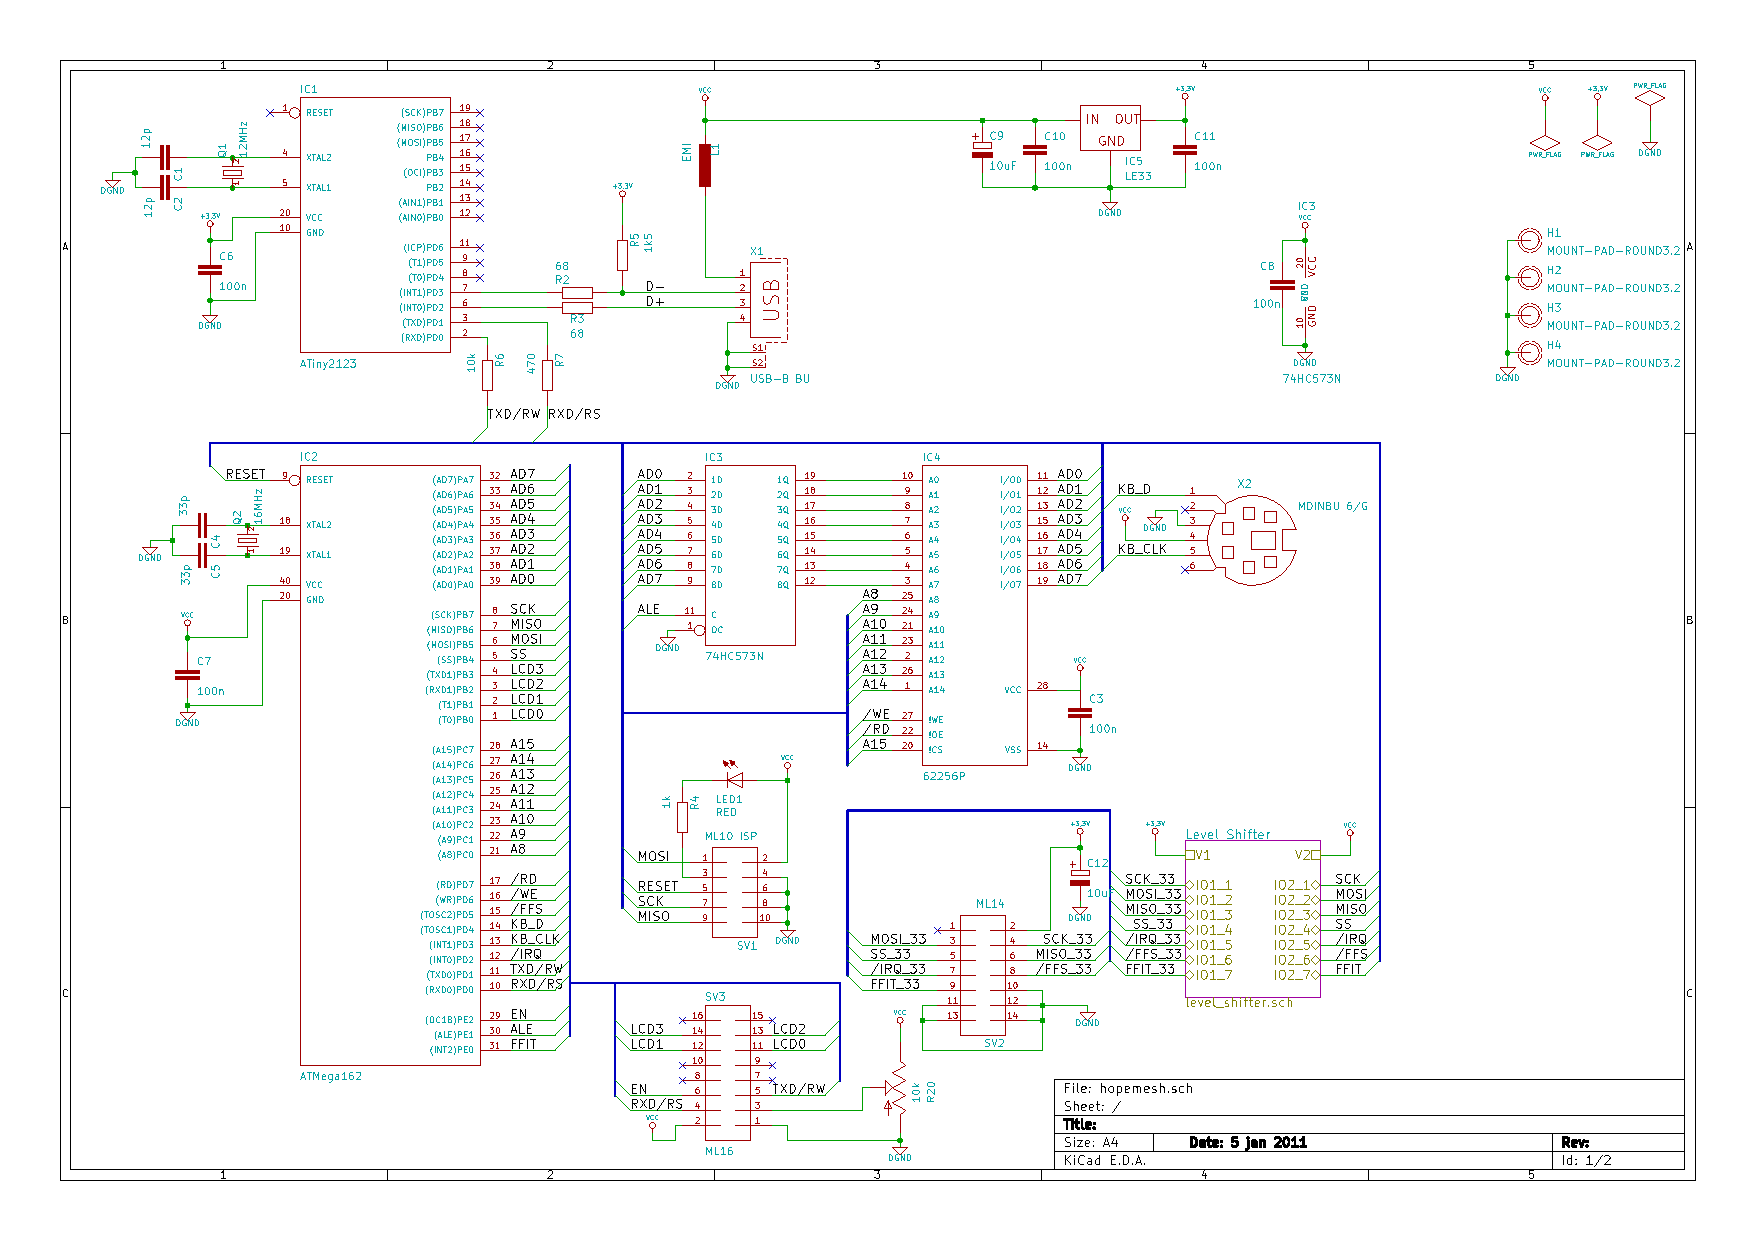
\includepdf[
    landscape,
    addtolist={
        1,
        figure,
        HopeMesh schematic,
        fig:hopemesh-sch
    }
]{figures/hopemesh-sch.pdf}

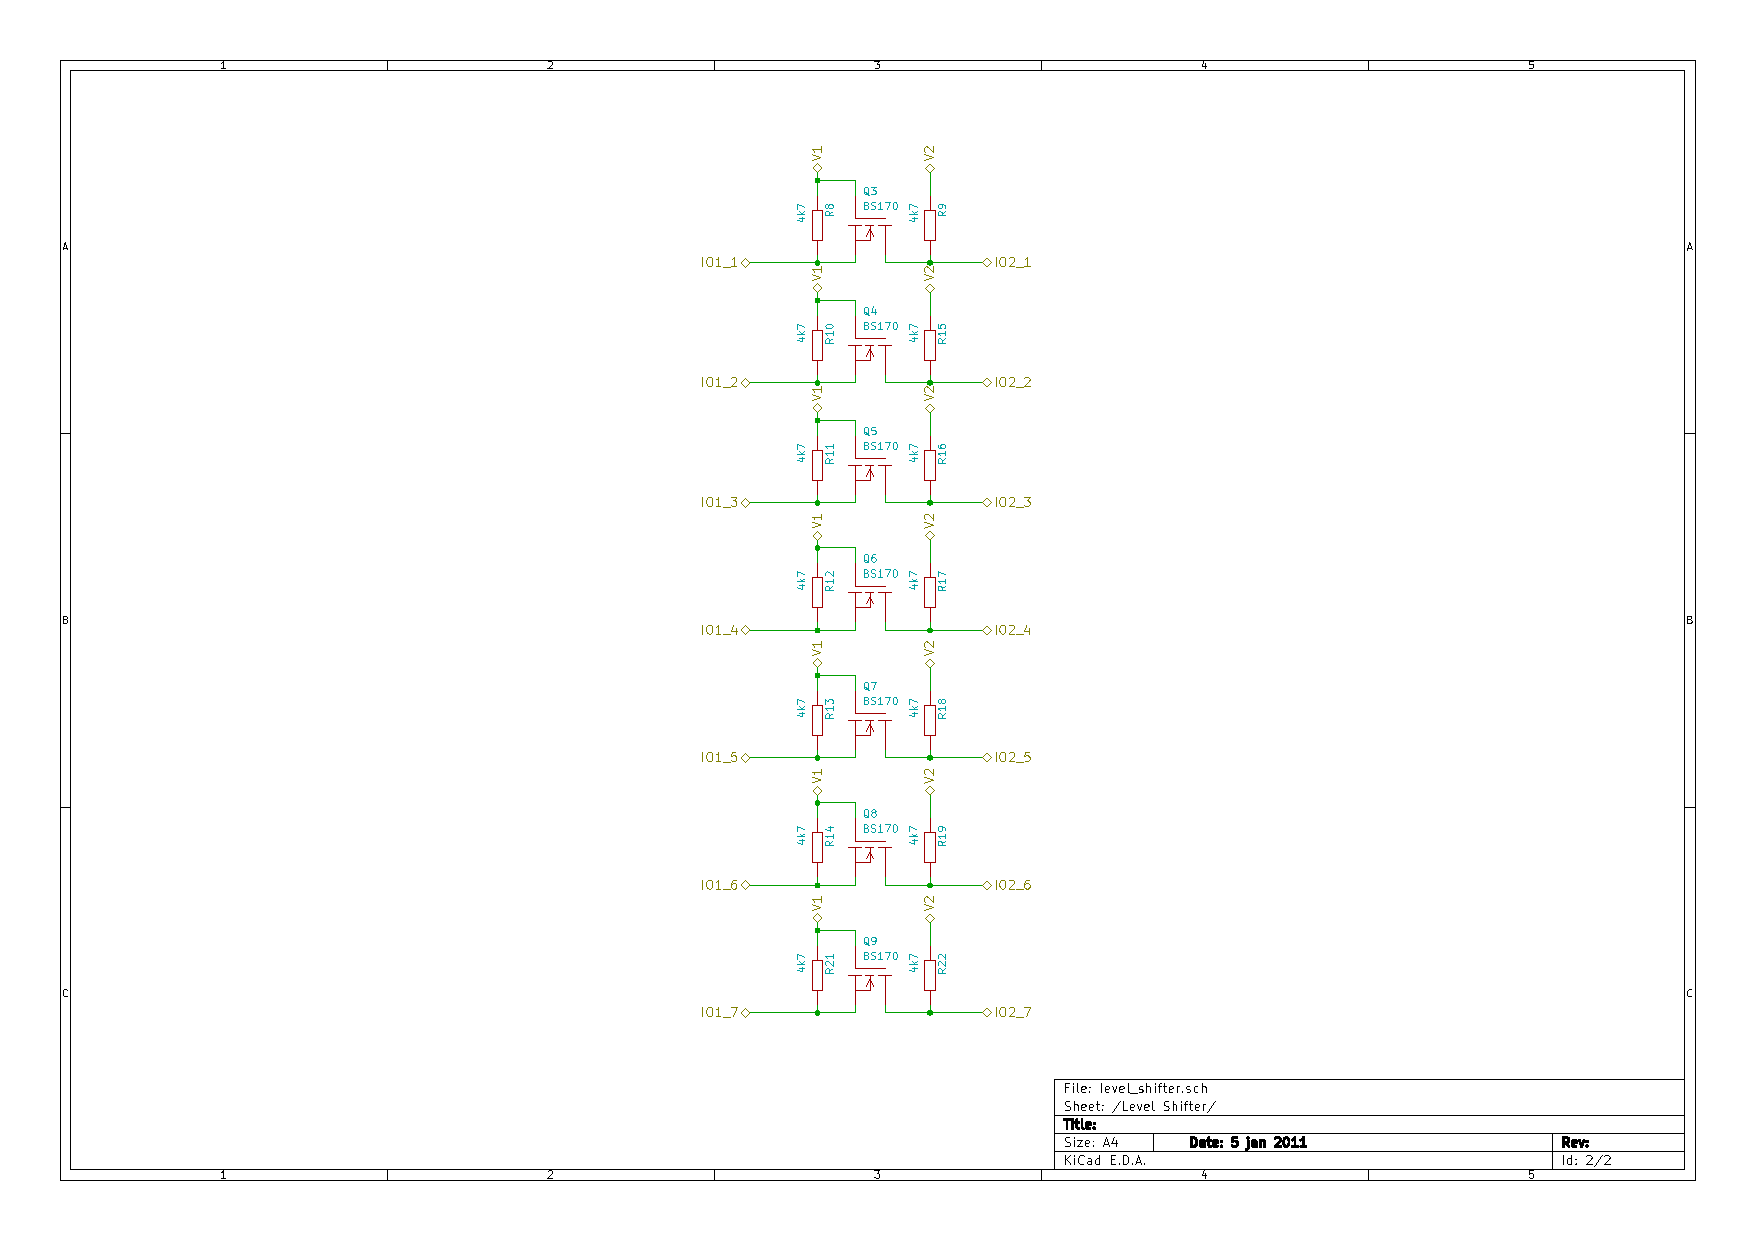
\includepdf[
    landscape,
    addtolist={
        1,
        figure,
        HopeMesh level shifter schematic,
        fig:hopemesh-sch-levelshifter
    }
]{figures/hopemesh-sch-levelshifter.pdf}

\section{Printed Circuit Board}
\begin{figure}[H]
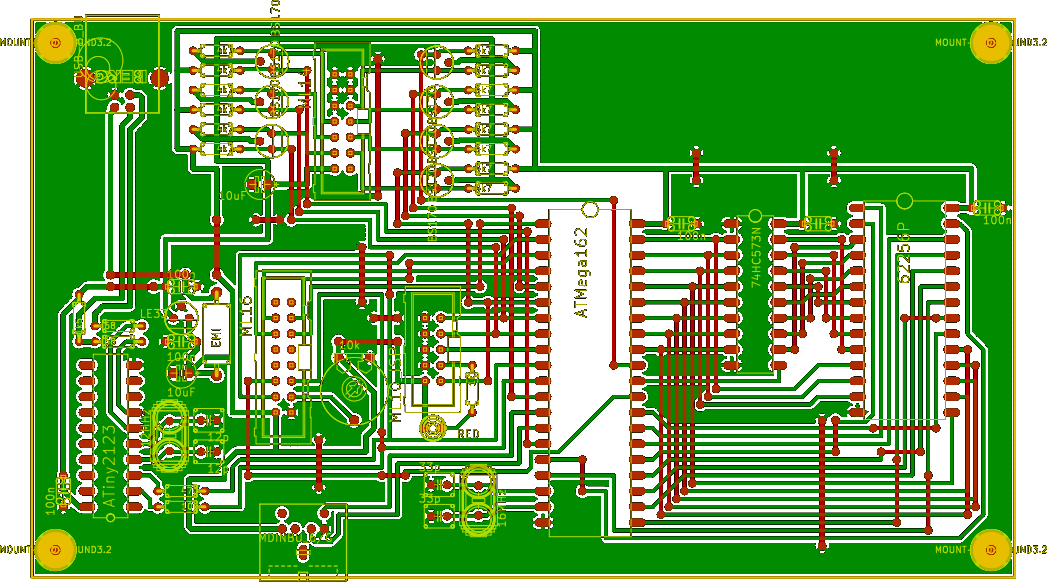
\includegraphics[width=\textwidth]{figures/2nd_rev_pcb_layout.png}
\caption{2nd revision PCB layout}
\end{figure}

In order to able to set up future mesh nodes a reproducable hardware design had to designed. The goal was to be able to produce many mesh nodes and to be able to equip a whole laboratory. One possibility is to manually wire each mesh node. Due to the complexity of the schematic this solution was not acceptable. The author decided to design a printed circuit board (PCB) in order to be able to produce new mesh nodes quickly. The following design requirements were established by the author:

\begin{itemize}
\item \textbf{One sided PCB: } The PCB was aimed to be manufactured in an uncomplicated environment. Two-sided PCBs allow minimizing the physical size of the device but for research this is not an important requirement. On the other hand two-sided PCBs require additional effort. Through-holes have to be manufactured and eventually the upper side of the PCB has to be laminated in order to prevent shorts.
\item \textbf{Non-SMD parts: } The author explicitly avoided SMD parts. The goal was to be able to solder the parts manually with commonly available electronic parts.
\end{itemize}

The actual design of the PCB (Printed Circuit Board) was performed in three iterative phases:
\begin{itemize}
\item \textbf{Manually wired prototype :} In order to have a proof of concept a first working prototype was constructed by the author manually. This board was not used for the final realization but was used in order to test the external RAM as well as the UART-USB connection.
\item \textbf{1st revision PCB :} A first revision of the PCB was designed and manufactured. Despite a function node a few design improvements were identified. The trace count and surface mounting the existing resistors were identified as a further improvement.
\item \textbf{2nd revision PCB :} The final revision of the PCB was designed in smaller dimensions and the design flaws from the first revision were corrected.
\end{itemize}

\begin{figure}[H]
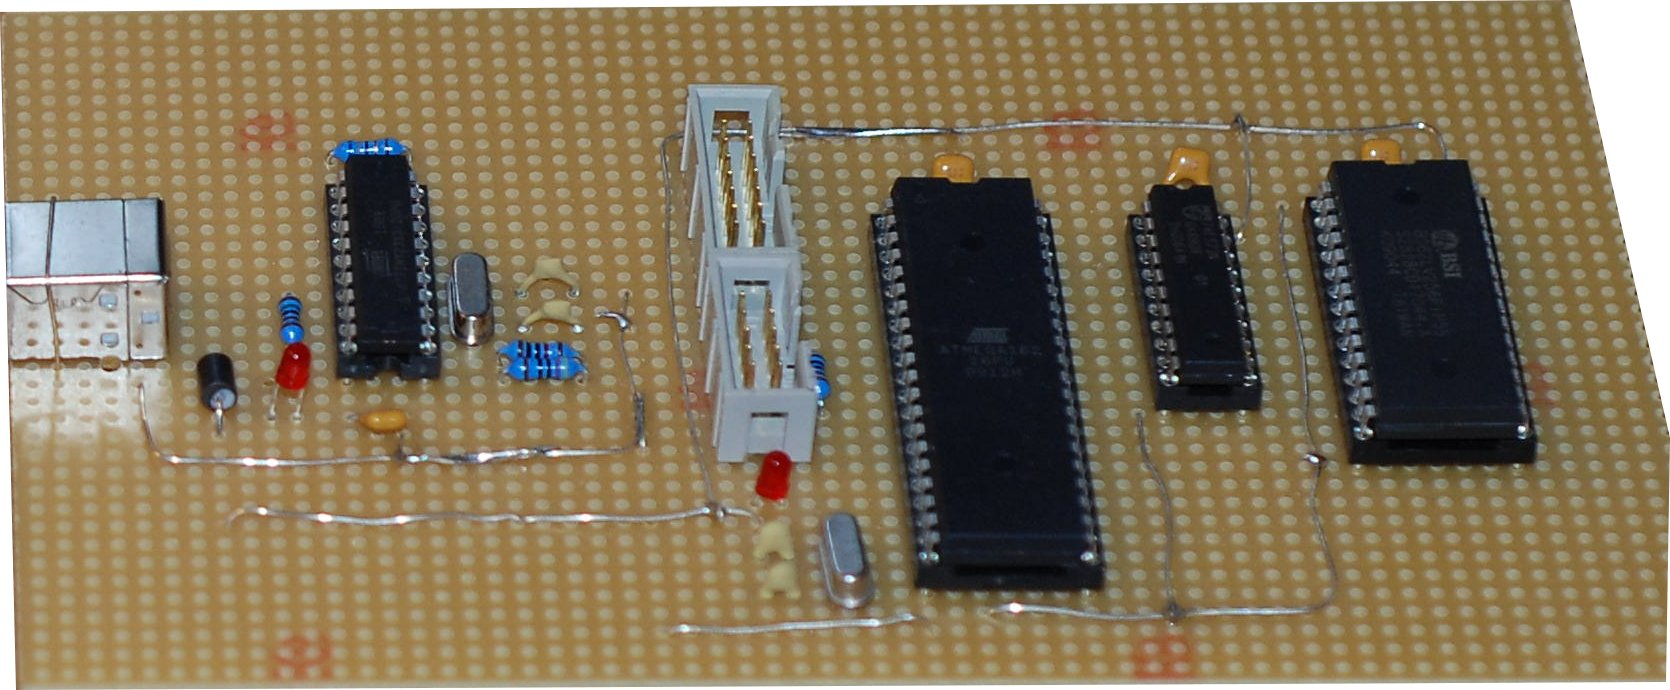
\includegraphics[width=\textwidth]{figures/prototype_pcb.jpg}
\caption{Manually wired prototype board}
\end{figure}

\begin{figure}[H]
    \centering
    \import{figures/}{2nd_rev_pcb.pdf_tex}
    \caption{2nd revision PCB areas}
\end{figure}

\chapter{Software Modules}
\section{UART}
\section{SPI}
\section{Watchdog}
\section{Timer}
\section{Shell}
\section{Network Stack}
\section{RFM12 Driver}

\chapter{Software Algorithms}
\section{Module orchestration}
Designing a software system that executes on embedded micro-controllers implies a lot of challenges when many software modules are involved and complexity grows. The conceptually defined modules must be somehow implemented. If the micro-controller lacks an operating system then there is no possibility of using provided abstractions and APIs for module orchestration and execution. Another challenge are limited hardware resources which prevent the deployment of many existing operating system kernels. Basically there are two types of execution models which can be implemented in micro-controllers:

\begin{enumerate}

\begin{figure}[H]
    \centering
    \import{figures/}{sequential_execution.pdf_tex}
    \caption{Sequential execution model}
\end{figure}

\item \textbf{Sequential execution model:} This type sequentially executes all modules inside an infinite main loop starting from the first module until the last one. Once the last module ends the execution starts again from the first module.

\begin{figure}[H]
\centering
\import{figures/}{concurrent_execution.pdf_tex}
\caption{Concurrent execution model}
\end{figure}
\item \textbf{Concurrent execution model:} This type executes modules concurrently. Instead of having an infinite main loop that iterates sequentially over all modules the main function only initializes and launches concurrent modules.
\end{enumerate}

\subsection{Sequential execution}
This model does not necessarily needs operating system support or frameworks. It can be simply implemented as a sequence of function calls inside an infinite loop as shown in algorithm \ref{alg:sequential execution}.

\begin{algorithm}[H]
\caption{Sequential model algorithm}
\label{alg:sequential execution}
\begin{algorithmic}
\WHILE{$true$}
\STATE $module_1$
\STATE $module_2$
\STATE $...$
\STATE $module_n$
\ENDWHILE
\end{algorithmic}
\end{algorithm}

There is one challenge that comes with this type of execution model. That is that only one module can execute at a time due to its sequential nature. If a module i.e. waits for an external resource to provide data it must not block the execution of the main loop until the external resources becomes ready. This would prevent the execution of the other modules. The classic solution to this problem is the introduction of states in modules. Module states can be implemented as classical Finite State Machines (\cite{booth}).

If we take the example from above about waiting for external resources a finite state machine for modules can be modeled as shown in figure \ref{fig:statemachine}.

\begin{figure}[H]
\centering
\import{figures/}{state_machine.pdf_tex}
\caption{State Machine for a module}
\label{fig:statemachine}
\end{figure}

State machine models can be implemented using \texttt{if} or \texttt{case} statements which is shown in algorithm \ref{alg:statemachine}. The nice side effect of a state machine based implementation is the non-blocking nature of the module execution. Take for instance the execution of state 1 "Waiting" as shown in figure \ref{fig:statemachine}. The CPU only needs to execute as many instructions as are necessary to check if the awaited resource is available. If the resource is not available the execution returns to the main loop and the next module (together with its state machine) is being executed.

\begin{algorithm}[H]
\caption{State machine algorithm}
\label{alg:statemachine}
\begin{algorithmic}
\IF{state is WAITING}
    \IF{resource is available}
        \STATE set state to PROCESSING
    \ELSE
        \STATE exit module
    \ENDIF
\ELSIF{state is PROCESSING}
    \STATE process data
    \STATE set state to WAITING
\ENDIF
\end{algorithmic}
\end{algorithm}

This implementation emulates a concurrent execution of modules. The context switch between module executions is being done by the modules themselves (using self-interruption) and no external scheduler is involved. This form of concurrent behavior can therefore be described as a non-preemptive or cooperative multi-tasking between modules. The predecessor thesis \cite{korniowski} implementation heavily used the described state machine algorithm although the model theory behind the implementation was not being mentioned in the thesis. Listing \ref{lst:korniowski_main} shows the main function of the predecessor implementation.

\begin{lstlisting}[
	label=lst:korniowski_main,
	caption=main loop routine (see \cite{korniowski})]
382 while(0x01)
383 {
384         if(uartInterrupt == ON) // got a character from RS232
385 +---- 44 lines: 
429 
430 
431         // --- RECEIVE A DATAGRAM ---
432 
433         else if((datagramReceived = datagramReceive(...)) 
                    && netState > 0)     
434 +----182 lines: 
616 
617     
618         else if(helloTime) // prepare periodic Hello message
619 +---- 19 lines: 
638 
639 
640     
641         // --- SEND A DATAGRAM ---
642     
643         if(datagramReady && netState > 0)
644 +----  8 lines: 
652 
653 }
\end{lstlisting}

A couple of problems arise from the existing implementation. First of all listing \ref{lst:korniowski_main} reveals the following modules:

\begin{itemize}
\item UART Module
\item Datagram Receiver Module
\item Hello Message Sender Module
\item Datagram Sender Module
\end{itemize}

Which module is being executed depends on the state of the main module being represented by the main function. The state of the main module on the other hand depends directly from the state of the submodules. The main module therefore acts more like a controller of the submodules and takes away the responsibility of the submodule's state management. Furthermore the main function is very long and complex (271 lines of code). Therefore the following goals were defined by the author:

\begin{itemize}
\item Clear separation of responsibilities between the main loop and the concurrently running modules.
\item Simplification of the main loop implementation.
\end{itemize}

Listing \ref{lst:urbaniak_main} shows the new implementation of the main loop. The new implementation makes it very clear which modules are being executed sequentially. Furthermore the main function does not act as a controller but rather leaves the state management in the module's responsibility.

\begin{lstlisting}[label=lst:urbaniak_main,caption=main function implementation]
 95 while (true) {
 96   shell();
 97   batman_thread();
 98   rx_thread();
 99   uart_tx_thread();
100   watchdog();
101   timer_thread();
102 }
\end{lstlisting}

The next question was how to implement the actual concurrently running modules. One possibility was to reuse the predecessor's methodology and use state machine based implementations. There is a problem though in state machine based implementations and that is the rapidly growing complexity. This problem is called "state explosion problem" and has even a exponential behavior as shown in \cite{katoen}. The equation \ref{eq:state explosion} shows that the number of states is dependent on the number of program locations, the number of used variables and their dimensions.

\begin{equation}
\label{eq:state explosion}
\#states = \abs{\#locations} \cdot \prod_{variable \: x} \: \abs{dom(x)}
\end{equation}

This equation shows that for instance a program having 10 locations and only 3 boolean variables already has 80 different states. Although this equation might not apply exactly to state machine based implementations it underlines the practical experience of big state-machine based implementations. The alternative to state-machine based applications are thread or process based implementations using the concurrent execution model as shown below.

\subsection{Concurrent execution}
This model requires support from an existing operating system. An existing framework or API provides the necessary abstraction to create new concurrent modules. Each module runs in isolation and can have its own main loop or terminate immediately. In terms of operating systems two abstractions are widely used for concurrently running software modules:

\begin{itemize}
\item \textbf{Processes}: Processes are usually considered as separately concurrently running programs. Usually each process owns its own memory context and communication with other processes happens through abstractions like pipes or shared memory.
\item \textbf{Threads}: Threads are concurrently running code parts from the same program. The initial program is considered to run in its own "main thread". Other threads can be started from the main thread. Threads also do run in isolation to each other. Each thread has its own stack. Communication with other threads happens through shared memory provided by static data or the heap.
\end{itemize}

Processes as well as threads are widely known concepts in classical desktop operating systems. In the area of embedded micro-controllers these concepts also are implemented in many different implementations:

\begin{enumerate}
\item FreeRTOS (http://www.freertos.org)
\item TinyOS (http://www.tinyos.net)
\item Atomthreads (http://http://atomthreads.com)
\item Nut/OS (http://www.ethernut.de/en/firmware/nutos.html)
\item BeRTOS (http://www.bertos.org)
\end{enumerate}

The above solutions have chosen different names for threads or processes (some call them "tasks") but essentially they all share the same concept of the concurrent execution model and will be referred to as concurrent modules from now on. Algorithm \ref{alg:threads} shows the pseudo-code that initializes concurrent modules. One can see that in contrast to the sequential execution model the main loop actually does nothing.

\begin{algorithm}[H]
\caption{Concurrent model initialization}
\label{alg:threads}
\begin{algorithmic}

\STATE start $module_1$
\STATE start $module_2$
\STATE ...
\STATE start $module_n$

\WHILE{true}
    \STATE // no operation
\ENDWHILE
\end{algorithmic}
\end{algorithm}

But how does a context switch happen between concurrent modules? Two methodologies exist:

\begin{itemize}
\item \textbf{Cooperative}: The concurrent modules by themselves return the control to a scheduler which then delegates the control to a different module. Which concurrent module gets control is often based on priorities which are controlled by the scheduler.
\item \textbf{Preemptive}: Here the concurrent modules do not have control about how and when they get interrupted. It can happen anytime during the execution. Again the context switch between concurrent modules is often handled using priorities in the scheduler.
\end{itemize}

Nearly all existing solutions have one feature in common. That is that every thread has its own separate stack memory space. This is necessary in order to be able to run the same block of code (for instance a function) in multiple thread instances. On the other hand threads are being executed in the same memory context so sharing data between threads is possible by using the heap or static memory. All of the above mentioned frameworks provide common abstractions which are needed in thread based implementations:

\begin{itemize}
\item Semaphores
\item Mutexes
\item Yielding
\end{itemize}

In contrast to state machine based or sequential based concurrency thread based implementation can be expressed in very linear algorithms using the above mentioned abstractions. Take for instance the state-machine based algorithm \ref{alg:statemachine}. This could be translated into a linear thread-based algorithm as shown in \ref{alg:thread}.

\begin{algorithm}[H]
\caption{Thread based algorithm}
\label{alg:thread}
\begin{algorithmic}
\WHILE{true}
    \STATE wait for resource mutex
    \STATE process data
    \STATE release resource mutex
\ENDWHILE
\end{algorithmic}
\end{algorithm}

One can easily see that the thread-based algorithm \ref{alg:thread} is much more expressive than the state-machine based algorithm \ref{alg:statemachine}.

Together with the necessity of having a scheduler these solutions can be considered as heavy-weight. The scheduler consumes additional CPU cycles and the separate stack memory space per thread consumes additional memory which is very scarce in embedded micro-controller systems.

Although usually a concurrent execution model must be provided in form of an API or an existing kernel there is one exception in the context embedded micro-controllers and that are ISRs (Interrupt Service Routines). Interrupt service routines behave like \emph{preemptive} concurrent modules with highest priority.

\begin{figure}[H]
\centering
\import{figures/}{isr.pdf_tex}
\caption{Illustration of an Interrupt Service Routine}
\end{figure}

The ISR interrupts the main program at any time when an external resource triggers an event and executes the service routine. The scheduler in this case is the CPU itself. There is one caveat with ISRs. When one ISR is being executed no other ISR can be triggered. Therefore it is being considered best practice not to perform intense and long running operations in ISRs.

\subsection{Conclusion}
For the implementation of this thesis the following conclusions were drawn:

\begin{itemize}
\item Existing solutions supporting the concurrent execution model were considered too heavy-weight for this type of application. Although 32KB of RAM are available the purpose is the support of route storage and network support.
\item A sequential execution model was favored instead of the concurrent execution model. On the other hand thread-like linear algorithms are definitely favored instead of state machine based implementations which could lead to a state explosion.
\end{itemize}

One framework exists which implements the sequential execution model but providing a linear thread-like API being called Protothreads as described in \cite{dunkels}. It is implemented using C macros and expands to switch statements (or to goto statements if the GCC compiler is being used). Instead of consuming a complete stack per thread the protothread implementation uses only two bytes per (proto)thread. Protothreads actually are stackless and variables initialized on the stack of a protothread function will stay initialized only during the very first call of the protothread.

\begin{algorithm}[H]
\caption{Simple linear algorithm}
\label{alg:linear}
\begin{algorithmic}
\WHILE{true}
    \STATE wait until timer expired
    \STATE process data
\ENDWHILE
\end{algorithmic}
\end{algorithm}

Algorithm \ref{alg:linear} shows a very simple linear use case where it waits for an external resource. In this case it waits for the expiration of an external timer by merely watching the timer's state. Since this is a read-only operation no explicit mutual exclusion is needed. This algorithm expressed as a protothread implementation is shown in listing \ref{lst:linear_protothread}.

\begin{lstlisting}[label=lst:linear_protothread,caption=linear protothread implementation]
 19 PT_THREAD(test(void))
 20 {
 21   PT_BEGIN(&pt);
 22   PT_WAIT_UNTIL(&pt, timer_ready());
 23   process_data();
 24   PT_END(&pt);
 25 }
\end{lstlisting}

The implementation of the algorithm is self-describing and corresponds to the APIs known from the concurrent execution model. The expanded version of the listing after the preprocessor stage is seen in \ref{lst:linear_protothread_expanded}.

\begin{lstlisting}[
  label=lst:linear_protothread_expanded,
  caption=expanded linear protothread implementation
]
char
test(void)
{
  // PT_BEGIN
  switch((&pt)->lc) {
    case 0:

      // PT_WAIT_UNTIL
      do {
        (&pt)->lc = 22;
    case 22:
        if(!(timer_ready())) {
          return 0;
        }
      } while(0);

      process_data();
  // PT_END
  };
  (&pt)->lc = 0;
  return 3;
}
\end{lstlisting}

The expanded version after the preprocessor stage of the implementation looks much more like a state machine based implementation from the sequential execution model. It uses a clever trick called loop unrolling (\cite{abrash}) which breaks ups the while statement using the switch statement. This technique is also known as Duff's device as described in \cite{duff}. Unfortunately this implementation has one drawback. One cannot (obviously) use switch statements in protothreads. A slightly more efficient implementation using GCC labels circumvents this. Since the context switch is managed by the concurrent modules themselves the behavior can be classified as \emph{cooperative} multitasking.

Due to the lightweight nature of protothreads and the possibility to express algorithms in a linear thread-like fashion this framework was chosen by the author for the implementation.

\section{Ring Buffers}
The predecessor thesis \cite{korniowski} used the UART interface in order to communicate with the user and to inform about incoming packets, changes to routes, etc.. As already analyzed in the previous chapter a state machine based sequential concurrent model was used to implement the UART module. There exists one problem with the current implementation.

\begin{lstlisting}[
	float,
	label=lst:korniowski_uart,
	caption=Sender route for the UART module (see \cite{korniowski})]
void rsSend(uint8_t data)
{
  while( !(UCSRA & (1<<UDRE)));
  UDR = data;
}
\end{lstlisting}

Listing \ref{lst:korniowski_uart} shows that the algorithm examines the UCSRA (USART Control and Status Register A) and blocks infinitely until the UDRE (USART Data Register Empty) bit becomes zero. The execution of all other concurrent modules and the main loop will be blocked until the UART becomes ready to accept data. In this time period no data can be received from the radio. The above mentioned implementation uses the same function for sending strings via the UART interface. For sending the string "hello" via the UART with a speed of 19.2kbps the main loop will be physically blocked for 2.5 milliseconds. In order to improve the implementation the author wanted to accomplish the following goals:

\begin{itemize}
\item Refactoring to a non-blocking operation.
\item Migration to a concurrent execution model using protothreads.
\end{itemize}

The Atmega162 micro-processor offers the following ISRs for receiving and sending data via the UART (\cite{atmega162datasheet}):

\begin{itemize}
\item \textbf{SIG\_USART\_RECV}: Is being invoked, when the UDR register contains a new byte received from the UART.
\item \textbf{SIG\_USART\_DATA}: Is being invoked, when the UDR register is ready to be filled with a byte to be transmitted via the UART.
\end{itemize}

So we have the possibility to send or receive data asynchronously from the main loop in the context of a concurrent execution model by using ISRs. Filling the UDR or reading the UDR in the main loop (and thus blocking it) is actually not necessary at all. The main loop can communicate with the ISRs through a receiving and transmitting queue buffer where it writes data to the transmitting queue and reads data from the receiving queue.

Using this sort of communication is known as the "producer-consumer problem". It can be implemented using a FIFO buffer. The Linux kernel (see \cite{linux_device_drivers} chapter 5.7.1) as well as (embedded) DSP micro-controllers (see \cite{ti_dsp}) use a very elegant FIFO-algorithm by providing a lock-free buffer being called "circular buffer" or "ring buffer".

\begin{figure}[H]
\centering
\import{figures/}{ringbuffer.pdf_tex}
\caption{Illustration of a ring buffer}
\label{fig:ringbuffer}
\end{figure}

Figure \ref{fig:ringbuffer} shows the basic principle of the algorithm. A circular buffer is defined by the following four pointers:

\begin{itemize}
\item \textbf{Start:} This pointer defines the beginning of the buffer in memory. This pointer is static.
\item \textbf{End:} This pointer defines the end of the buffer in memory. It can also be expressed as the maximum length of the buffer. This pointer is static.
\item \textbf{Head:} The head pointer is being changed dynamically by the producer. Whenever the producer wants to write data in the buffer the head pointer is increased and the corresponding memory filled. If the head points to the same address as the tail pointer the buffer is full or empty.
\item \textbf{Tail:} The tail pointer is being changed dynamically by the consumer. Whenever the consumer wants to read data from the buffer the tail pointer is increased and the corresponding memory cleared. If the tail points to the same address as the head pointer the buffer is full or empty.
\end{itemize}

In order to distinguish whether the buffer is full or empty an additional size variable was implemented. The biggest advantage of the presented algorithm is the possibility to write and read data in a lock-free fashion. A consumer thread does not need to wait for a mutual exclusion on the buffer since the consumer thread is the only instance manipulating the tail pointer. The same applies for the producer being the only instance manipulating the head pointer.

The complete listing of the ring-buffer implementation can be seen in appendix \ref{chapter:appendix_a} in the file \texttt{src/ringbuf.c}. There are two functions provided:

\begin{itemize}
\item \textbf{ringbuf\_add:} This function is being called by the producer. The function immediately returns \texttt{true} if a byte could be written to the the buffer or \texttt{false} if the buffer is full.
\item \textbf{ringbuf\_remove:} This function is being called by the consumer. The function immediately returns \texttt{true} if a byte could read from the buffer or \texttt{false} if the buffer is empty.
\end{itemize}

The important nature of the above mentioned functions is that they are non-blocking because they return immediately. These functions could therefore be called from protothreads. A producer protothread running in the context of the main loop can write data like presented in listing \ref{lst:producer_ringbuf}. The consumer of this data is the SIG\_USART\_DATA ISR as presented in listing \ref{lst:consumer_ringbuf}.

\begin{lstlisting}[
    label=lst:producer_ringbuf,
    caption=Producer writing data
]
PT_THREAD(producer(uint8_t data))
{
    PT_BEGIN(&pt);
    PT_WAIT_UNTIL(&pt, ringbuf_add(buf, data));
    PT_END(&pt);
}
\end{lstlisting}

\begin{lstlisting}[
    label=lst:consumer_ringbuf,
    caption=Consumer reading data
]
ISR(SIG_USART_DATA)
{
  uint8_t c;
  if (ringbuf_remove(buf, &c)) {
    UDR = c;
  }
}
\end{lstlisting}

Instead of \emph{physically} blocking the algorithm expressed in listing \ref{lst:producer_ringbuf} only \emph{logically} blocks the protothread. If the buffer is full a context-switch back to the main loop is performed. The main loop sequentially executes all other concurrent modules and returns to the protothread which then again tries to add data into the ring buffer.

\section{Half-Duplex Radio Access (Petri Net)}
The predecessor implementation used an identical (physically) blocking implementation in order to send or receive data via the RFM12B hardware module. Listing \ref{lst:rfm12b_predecessor_tx} shows the algorithm used for sending data.

\begin{lstlisting}[
    label=lst:rfm12b_predecessor_tx,
    caption=Sender routine for the RFM12B hardware module (see \cite{korniowski})
]
void rfTx(uint8_t data)
{
        while(WAIT_NIRQ_LOW());
        rfCmd(0xB800 + data);
}
\end{lstlisting}

This implementation physically blocks the main loop the same way as the UART algorithm shown in listing \ref{lst:korniowski_uart}. In this case the algorithm does not wait for the status of an internal register to send data but rather waits for the external nIRQ pin from the RFM12B hardware module to go low. The official "RF12B programming guide" (see \cite{rf12b_programming_guide}) also proposes a physically blocking algorithm.

The author wanted to improve the algorithm in a similar fashion as the UART algorithm. The nIRQ pin of the RFM12B was connected to the INT0 pin of the ATMega162 micro-processor allowing to execute the SIG\_INTERRUPT0 interrupt service routine asynchronously. But it turned out that the implementation could not be reused at all. The RFM12B radio hardware imposes the following algorithmic challenges for the driver implementation:
\begin{itemize}
\item \textbf{Single interrupt request for multiple events:} The RFM12 radio module uses only one nIRQ pin in order to generate an interrupt for the following events (see \cite{sis4221_datasheet}):
\begin{itemize}
\item The TX register is ready to receive the next byte (RGIT)
\item The RX FIFO has received the preprogrammed amount of bits (FFIT)
\end{itemize}
The state management has to be implemented in software otherwise the current state of operation (sending or receiving) is undefined.
\item \textbf{Half-Duplex operation:} The RFM12 radio module only allows either to receive or to send data at a time but not simultaneously.
\end{itemize}

The author abstracted the operation of the RFM12B driver algorithm as a (proto)thread. Interestingly enough the thread has a state modeled as a state machine depending whether it receives or sends data. The following states are valid:

\begin{itemize}
\item \textbf{RX:} This is the receiving state. The thread (logically) blocks until a complete packet has been received. Whether a packet is complete or not depends on the upper network stack layers.
\item \textbf{TX:} This is the sending state. The thread (logically) blocks until a complete packet has been sent. Again the upper network stack layers decide whether the transmission is complete or not.
\end{itemize}

The abstract algorithm is shown in \ref{alg:rfm12b_thread}. The question is who sets the actual state of the radio driver. Receiving data is \emph{non-deterministic}. A packet can arrive at any time and thus the invocation of the SIG\_INTERRUPT0 interrupt service routine. Therefore the algorithm sets the RX state as the \emph{default} state for the radio thread.

Sending data on the other hand is \emph{deterministic}. When a user hits the Enter key via the UART module a packet can be constructed. A 3rd party thread has to request the control over the radio module and occupy it until the packet has been fully transmitted. The author realized that this is a concurrency problem between two threads and a single resource:
\begin{itemize}
\item \textbf{Sender Thread:} The sender thread wants to acquire the control over the radio module until the transmission of a packet is complete.
\item \textbf{Radio Thread:} The radio thread also wants to acquire the control over the radio module until the packet reception is complete.
\item \textbf{Single resource:} The external resource in this case is the radio module. Only the receiving radio driver thread or the transmitting sender thread can own the radio hardware resource at a time.
\end{itemize}

\begin{algorithm}[H]
\caption{RFM12B driver thread algorithm}
\label{alg:rfm12b_thread}
\begin{algorithmic}
\WHILE{$true$}
    \IF{state is RX}
        \STATE receive data
    \ELSIF{state is TX}
        \STATE send data
    \ENDIF 

    \STATE set state to RX
\ENDWHILE
\end{algorithmic}
\end{algorithm}

In classical multi-threaded algorithms this problem can be solved using mutual exclusion. Modeling such an algorithm can be done using petri nets as shown in figure \ref{fig:petri_mutex}.

\begin{figure}[H]
\centering
\import{figures/}{mutex.pdf_tex}
\caption{Mutual exclusion model using a petri net}
\label{fig:petri_mutex}
\end{figure}

\begin{figure}[H]
\centering
\import{figures/}{rfm12_petri.pdf_tex}
\caption{Half duplex algorithm modeled as a petri net}
\end{figure}

\chapter{Network Stack}
\section{Layer 2a: MAC Layer}
\section{Layer 2b: Logical Link Control}
Hamming Code
\section{Layer 3: Batman Routing}
\section{Layer 7: Application}

\chapter{Research}
\section{Simulations}
\subsection{Shell}
\subsection{Routing}
\subsection{Radio Transmission}
\section{Mesh evaluation}
\section{Results}

\chapter{Conclusion}
